%Preamble
\documentclass[12pt]{article}
\usepackage{fancyhdr}
\usepackage{extramarks}
\usepackage{amsmath}
\usepackage{amssymb}
\usepackage{amsthm}
\usepackage{amsrefs}
\usepackage{amsfonts}
\usepackage{mathrsfs}
\usepackage{mathtools}
\usepackage[mathcal]{eucal} %% changes meaning of \mathcal
\usepackage{enumerate}
\usepackage[shortlabels]{enumitem}
\usepackage{verbatim} %% includes comment environment
\usepackage{hyperref}
\usepackage[capitalize]{cleveref}
\crefformat{equation}{~(#2#1#3)}
\usepackage{caption, subcaption}
\usepackage{graphicx}
\usepackage{fullpage} %%smaller margins
\usepackage[all,arc]{xy}
\usepackage{mathrsfs}

\hypersetup{
    linktoc=all,     % set to all if you want both sections and subsections linked
}

\topmargin=-0.45in
\evensidemargin=0in
\oddsidemargin=0in
\textwidth=6.5in
\textheight=9.0in
\headsep=0.25in
\setlength{\headheight}{16pt}

\linespread{1.0}

\pagestyle{fancy}
\lhead{\Name}
\chead{\hwClass: \hwTitle}
\rhead{\hwDueDate}
\lfoot{\lastxmark}
\cfoot{\thepage}

\renewcommand\headrulewidth{0.4pt}
\renewcommand\footrulewidth{0.4pt}

\setlength\parindent{0pt}

%% Title Info
\newcommand{\hwTitle}{HW \# 1}
\newcommand{\hwDueDate}{Jan 20, 2020}
\newcommand{\hwClass}{AMATH 568}
\newcommand{\hwClassTime}{}
\newcommand{\hwClassInstructor}{}
\newcommand{\Name}{\textbf{Marlin Figgins}}


%% MATH MACROS
\newcommand{\bbF}{\mathbb{F}}
\newcommand{\bbN}{\mathbb{N}}
\newcommand{\bbQ}{\mathbb{Q}}
\newcommand{\bbR}{\mathbb{R}}
\newcommand{\bbZ}{\mathbb{Z}}
\newcommand{\bbC}{\mathbb{C}}
\newcommand{\abs}[1]{ \left| #1 \right| }
\newcommand{\diff}[2]{\frac{d #1}{d #2}}
\newcommand{\infsum}[1]{\sum_{#1}^{\infty}}
\newcommand{\norm}[1]{ \left|\left| #1 \right|\right| }
\newcommand{\eval}[1]{ \left. #1 \right| }
\newcommand{\Expect}[1]{\mathbb{E}\left[#1 \right]}
\newcommand{\Var}[1]{\mathbb{V}\left[#1 \right]}
\renewcommand{\vec}[1]{\mathbf{#1}}

\renewcommand{\phi}{\varphi}
\renewcommand{\emptyset}{\O}

%--------Theorem Environments--------
%theoremstyle{plain} --- defaultx
\newtheorem{thm}{Theorem}[section]
\newtheorem{cor}[thm]{Corollary}
\newtheorem{prop}[thm]{Proposition}
\newtheorem{lem}[thm]{Lemma}
\newtheorem{conj}[thm]{Conjecture}
\newtheorem{quest}[thm]{Question}

\theoremstyle{definition}
\newtheorem{defn}[thm]{Definition}
\newtheorem{defns}[thm]{Definitions}
\newtheorem{con}[thm]{Construction}
\newtheorem{exmp}[thm]{Example}
\newtheorem{exmps}[thm]{Examples}
\newtheorem{notn}[thm]{Notation}
\newtheorem{notns}[thm]{Notations}
\newtheorem{addm}[thm]{Addendum}

% Environments for answers and solutions
\newtheorem{exer}{Exercise}
\newtheorem{sol}{Solution}

\theoremstyle{remark}
\newtheorem{rem}[thm]{Remark}
\newtheorem{rems}[thm]{Remarks}
\newtheorem{warn}[thm]{Warning}
\newtheorem{sch}[thm]{Scholium}

\makeatletter
\let\c@equation\c@thm
\makeatother

\begin{document}

For exercises 1-7, (a) determine the eigenvalues and eigenvectors and (b) sketch the behavior and classify the behavior. 

\begin{exer}
\begin{equation*}
\frac{d \vec{x}}{dt} 
=
\begin{pmatrix}
    2 & -5\\
    1 & -2
\end{pmatrix}
\vec{x}.
\end{equation*}
\end{exer}

\begin{sol}\leavevmode
Using $\det(\vec{A} - \lambda \vec{I})$, we'll solve for the eigenvalues of the above matrix. We see that
\begin{align*}
    (2 - \lambda)(-2 - \lambda) - 5 = 0 \implies \lambda_{1} = i, \lambda_{2} = -i.
\end{align*}
We can use these eigenvalues to solve for the eigenvectors as follows. Suppose that our $i$-th eigenvector is $\vec{v}_{i}$, then we have

\begin{align*}
\vec{A} \vec{v}_{i} = \lambda_{i} \vec{v}_{i}.
\end{align*}
Solving this for our first eigenvalue gives
\begin{align*}
    (2 - i) x = 5y \\
    x = (2 + i)y.
\end{align*}
For $y = 1$, this gives us the eigenvetor $\vec{v}_{1} = (2 + i, 1)^{T}$. Repeating this to find the second eigenvector, we get that

\begin{align*}
    (2 + i) x = 5y \\
    x = (2 - i)y,
\end{align*}
which gives $\vec{v}_{2} = (2 - i, 1)^{T}$. Since both eigenvalues are purely imaginary, we expect that the solution will be completely oscillatory.
 \end{sol}

 \begin{figure}[h]
     \centering
     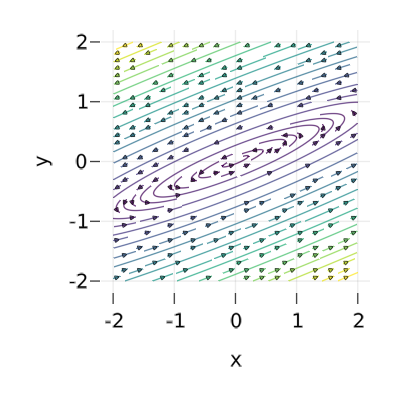
\includegraphics[width=0.8\linewidth]{figs/hw-1-exer-1.png}
     \caption{Plotting vector field for exercise 1.}%
     \label{fig:exer-1}
 \end{figure}

\newpage
 
\

\newpage

\begin{exer}
\begin{equation*}
\frac{d \vec{x}}{dt} 
=
\begin{pmatrix}
    -1 & -1\\
    0 & -0.25
\end{pmatrix}
\vec{x}.
\end{equation*}
\end{exer}

\begin{sol}\leavevmode
    We can repeat the same general method as before to solve for the eigenvalues and eigenvectors. We begin by computing the characteristic polynomial $\det( \vec{A} - \lambda \vec{I} )$  of the above matrix and finding its zeroes
    \begin{equation*}
        (1-\lambda)(- 1 / 4 - \lambda) = 0 \implies \lambda_{1} = -1, \lambda_{2} = - \frac{1}{4}.
    \end{equation*}
    Using the same form to compute the eigenvectors, we arrive at the following system of equations for our first eigenvalue
    \begin{align*}
    - x - y = - x\\
    - y / 4  = - y,
    \end{align*}
    which implies $y = 0$, so $\vec{v}_{1} = (1, 0)^{T}$. Repeating for the second set, we seee that
    \begin{align*}
    -x - y = - x /4  \\
    - y / 4  = - y / 4 .
    \end{align*}
    Picking $y = 1$, we get our second eigenvector as $\vec{v} = (- 3 / 4 , 1)^{T}$. Since both eigenvalues are real and negative, we expect there to be a stable fixed point.
 \end{sol}

\begin{figure}[h]
     \centering
     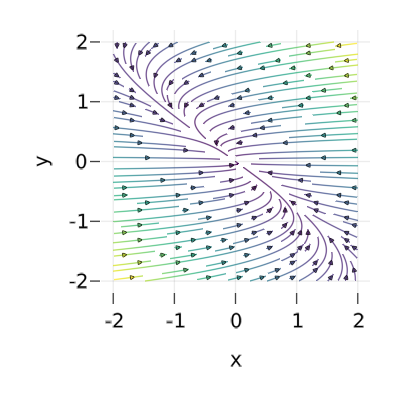
\includegraphics[width=0.8\linewidth]{figs/hw-1-exer-2.png}
     \caption{Plotting vector field for exercise 2.}%
     \label{fig:exer-2}
\end{figure}

\newpage
 
\

\newpage

\begin{exer}
\begin{equation*}
\frac{d \vec{x}}{dt} 
=
\begin{pmatrix}
    3 & -4\\
    1 & -1
\end{pmatrix}
\vec{x}.
\end{equation*}
\end{exer}

\begin{sol}\leavevmode
    We write the characteristic polynomial and solve for its zeroes 
    \begin{align*}
        (3 - \lambda)(-1 - \lambda) + 4 = 0 \implies \lambda = 1
    \end{align*}
    which is a double root. In this case, we also solve for the eigenvector(s), and find there is only one eigenvector which is given by
    \begin{align*}
    3x - 4y = x\\
    x - y = y,
    \end{align*}
    for $y = 1$, we see this is simply $\vec{v} = (2, 1)^{T}$. In this case, our solution depends on the generalized eigenvector, but we can still easily classify this as an improper unstable node since $\lambda > 0$.
 \end{sol}

  \begin{figure}[h]
     \centering
     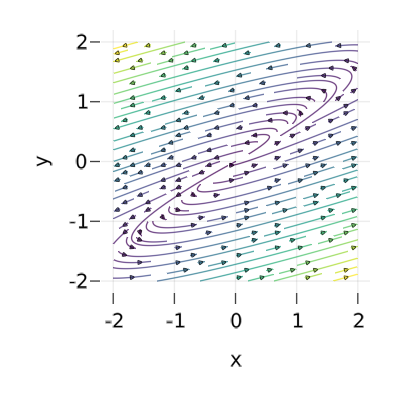
\includegraphics[width=0.8\linewidth]{figs/hw-1-exer-3.png}
     \caption{Plotting vector field for exercise 3.}%
     \label{fig:exer-3}
 \end{figure}


\newpage

\

\newpage

\begin{exer}
\begin{equation*}
\frac{d \vec{x}}{dt} 
=
\begin{pmatrix}
    2 & -5 / 2\\
    9 / 5 & -1
\end{pmatrix}
\vec{x}.
\end{equation*}
\end{exer}

\begin{sol}\leavevmode
     We write the characteristic polynomial and solve for its zeroes
     \begin{align*}
         (2 - \lambda) (-1 - \lambda) + 9 / 2 = 0 \implies \lambda_{1,2} = \frac{1}{2} \pm \frac{3}{2} i.
     \end{align*}
     We can solve for the corresponding eigenvector using the first eigenvalue so that 
     \begin{align*}
         2x - \frac{5y}{2}=  (\frac{1}{2} + \frac{3}{2}i )x\\
    \frac{9x}{5} - y = (\frac{1}{2} + \frac{3}{2}i)y
     \end{align*}
     Setting $y = 6$, we see that our eigenvector will be given by $\vec{v}_{1} = (5 + 5i, 6)^{T}$ after a bit of algebra. As the matrix is real and the eigenvalues are a conjugate pair, we know the second eigenvector must be given by $\vec{v}_{2} = \overline{\vec{v}_{1}} = (5 - 5i, 6)^{T}$. As both eigenvalues are complex with positive real part, we know expect there to be an outward spiral.
 \end{sol}

  \begin{figure}[h]
     \centering
     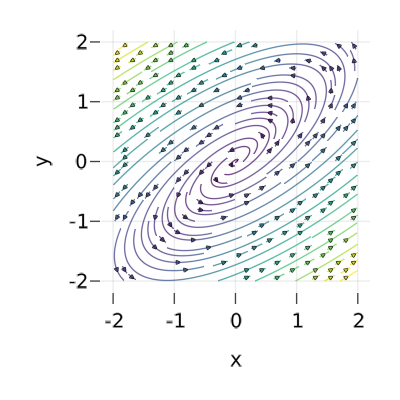
\includegraphics[width=0.8\linewidth]{figs/hw-1-exer-4.png}
     \caption{Plotting vector field for exercise 4.}%
     \label{fig:exer-4}
 \end{figure}

\newpage


\

\newpage

\begin{exer}
\begin{equation*}
\frac{d \vec{x}}{dt} 
=
\begin{pmatrix}
    2 & -1\\
    3 & -2
\end{pmatrix}
\vec{x}.
\end{equation*}
\end{exer}

\begin{sol}\leavevmode
    Writing the characteristic polynomials and finding zeroes,
    \begin{align*}
        (2 - \lambda) ( - 2 - \lambda ) + 3 = 0 \implies \lambda_{1,2} = \pm 1.
    \end{align*}
    Setting up the equations for the first eigenvalue, we see that

    \begin{align*}
    2 x - y = x\\
    3x - 2y = y
    \end{align*}
    From these, we see that $x = y$, so our first eigenvector is $\vec{v}_{1} = (1, 1)^{T}$. Solving for the second eigenvector
    \begin{align*}
    2 x - y = -x\\
    3x - 2y = -y,
    \end{align*}
    setting $y = 3$, we see that $x = 1$, so that $\vec{v}_{2} = (1,3)^{T}$. We have real eigenvalues one of which is positive and the other of which is negative so we expect a saddle point.
 \end{sol}

  \begin{figure}[h]
     \centering
     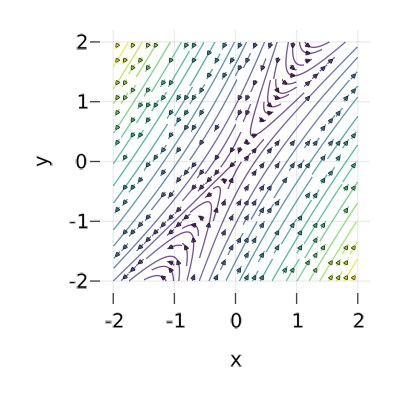
\includegraphics[width=0.8\linewidth]{figs/hw-1-exer-5.png}
     \caption{Plotting vector field for exercise 5.}%
     \label{fig:exer-5}
 \end{figure}

\newpage

\

\newpage

\begin{exer}
\begin{equation*}
\frac{d \vec{x}}{dt} 
=
\begin{pmatrix}
    1 & \sqrt{3}\\
    \sqrt{3} & -1
\end{pmatrix}
\vec{x}.
\end{equation*}
\end{exer}

\begin{sol}\leavevmode
    Writing the characteristic polynomials and finding zeroes,
    \begin{align*}
        (1 - \lambda)(-1 - \lambda) - 3 = 0 \implies \lambda_{1,2} = \pm 2.
    \end{align*}
    Setting up equations using the first eigenvalue, we see
    \begin{align*}
        x  + \sqrt{3} y = 2x\\
        \sqrt{3} x - y = 2y
    \end{align*}
    For $y = 1$, we see this reduces to $x = \sqrt{3}$ from the first of the above equations. Therefore our first eigenvector is $\vec{v}_{1} = (\sqrt{3}, 1)^{T}$ Repeating the second eigenvalue, we see
    \begin{align*}
        x  + \sqrt{3} y =-2x\\
        \sqrt{3} x - y = -2y
    \end{align*}
    This time setting $x = 1$, we see that $y = - \sqrt{3}$. Our second eigenvector is then $\vec{v}_{2} = (1, -\sqrt{3})^{T}$. Once again, we have two real eigenvalues one of which is negative and the other positive which is once again a saddle point.
 \end{sol}

  \begin{figure}[h]
     \centering
     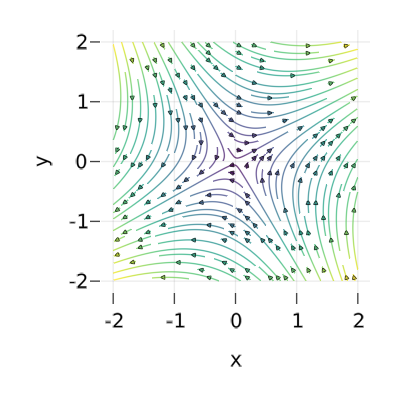
\includegraphics[width=0.8\linewidth]{figs/hw-1-exer-6.png}
     \caption{Plotting vector field for exercise 6.}%
     \label{fig:exer-6}
 \end{figure}

\newpage

\

\newpage 

\begin{exer}
\begin{equation*}
\frac{d \vec{x}}{dt} 
=
\begin{pmatrix}
    3 & -2\\
    2 & -2
\end{pmatrix}
\vec{x}.
\end{equation*}
\end{exer}

\begin{sol}\leavevmode
    Writing the characteristic polynomials and finding zeroes,
    \begin{align*}
        (3 -\lambda)(-2 - \lambda) + 4 = 0 \implies \lambda_{1} = 2, \lambda_{2} = 1.
    \end{align*}
    Setting up equations using the first eigenvalue, we see
    \begin{align*}
        3x  -2 y = 2x\\
        2x - 2y = 2y
    \end{align*}
    Setting $y = 1$, we see that $x = 2$, so our first eigenvector is $\vec{v}_{1} = (2,1)^{T}$. The second eigenvector is given by
    \begin{align*}
        3x  -2 y = -x\\
        2x - 2y = -y
    \end{align*}
    This time setting $x = 1$, we see that $y = 2$, so that our second eigenvector is given by $\vec{v}_{2} = (1, 2)^{T}$. We have two real eigenvalues one of which is positive and the other of which is negative which gives another saddle point.
 \end{sol}

  \begin{figure}[h]
     \centering
     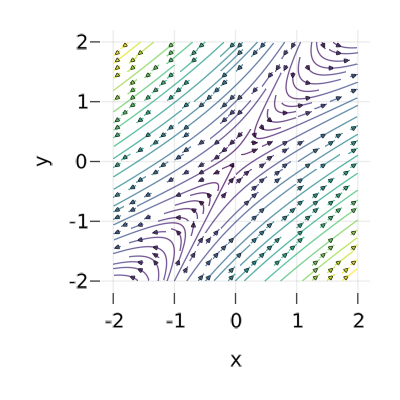
\includegraphics[width=0.8\linewidth]{figs/hw-1-exer-7.png}
     \caption{Plotting vector field for exercise 7.}%
     \label{fig:exer-7}
 \end{figure}

\newpage

\

\newpage


\begin{exer}
Consider 
\begin{align*}
    \frac{dx}{dt} &= - (x - y) (1 - x - y)\\
    \frac{dy}{dt} &=x( 2 + y )
\end{align*}
and plot the solutions. Verify your qualitative dynamics with Julia.
\end{exer}

\begin{sol}\leavevmode
    I think this question is a bit unclear.  I'll plot the vector fields associated with these as before using Julia and also simulate some example trajectories. From the vector field plotted below and the system of equations above, there appear to be two fixed points one of which is stable and the other which is unstable. These two fixed points are $(x,y) = (0,1)$ and $(x,y) = (0,0)$ respectively.
 \end{sol}

   \begin{figure}[h]
     \centering
     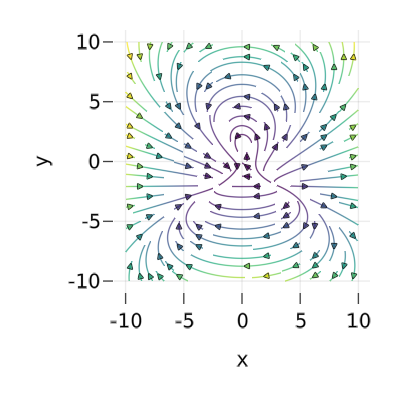
\includegraphics[width=0.8\linewidth]{figs/hw-1-exer-8.png}
     \caption{Plotting vector field for exercise 8.}%
     \label{fig:exer-8}
 \end{figure}

   \begin{figure}[h]
     \centering
     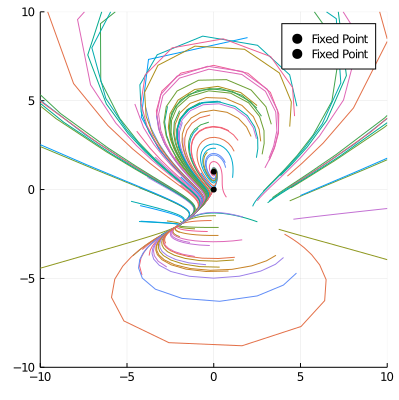
\includegraphics[width=0.8\linewidth]{figs/hw-1-exer-8-traj.png}
     \caption{101 simulated trajectories from exercise 8.}%
     \label{fig:exer-8-traj}
 \end{figure}

\newpage

\

\newpage

\begin{exer}
Consider 
\begin{align*}
    \frac{dx}{dt} &= x - y^2\\
    \frac{dy}{dt} &= y - x^2
\end{align*}
and plot the solutions. Verify your qualitative dynamics with Julia.
\end{exer}

\begin{sol}\leavevmode
    Here I only present the phase portrait as there were issues actually simulating the ODEs. I believe the solutions were blowing up too quickly. This system has fixed points when
    \begin{align*}
        x = y^{2} \text{ AND } y = x^2,
    \end{align*}
    which has two solutions $(x = 0, y = 0)$ and $x = 1, y = 1$. 
 \end{sol}

   \begin{figure}[h]
     \centering
     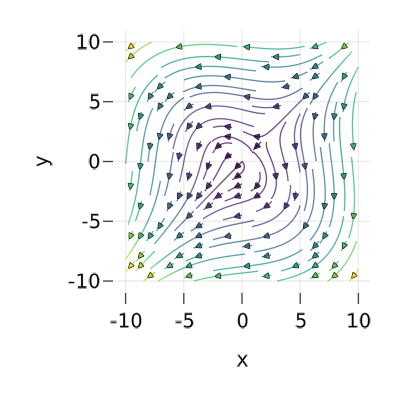
\includegraphics[width=0.8\linewidth]{figs/hw-1-exer-9.png}
     \caption{Plotting vector field for exercise 9.}%
     \label{fig:exer-9}
 \end{figure}

\newpage

\

\newpage

\begin{exer}
Consider 
\begin{align*}
    \frac{dx}{dt} &= (2 + x)(y - x)\\
    \frac{dy}{dt} &= (4 - x) ( y + x )
\end{align*}
and plot the solutions. Verify your qualitative dynamics with Julia.
\end{exer}

\begin{sol}\leavevmode
    We plot the vector field below as well as the phase portrait for several simulated trajectories. There are appears to be both a stable fixed point and an unstable fixed point here. 
 \end{sol}

   \begin{figure}[h]
     \centering
     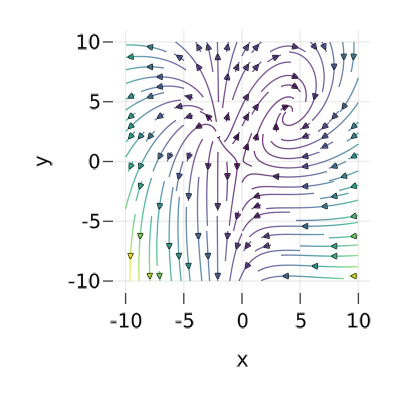
\includegraphics[width=0.8\linewidth]{figs/hw-1-exer-10.png}
     \caption{Plotting vector field for exercise 10.}%
     \label{fig:exer-10}
 \end{figure}

    \begin{figure}[h]
     \centering
     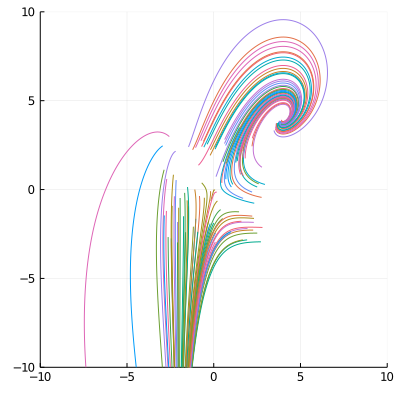
\includegraphics[width=0.8\linewidth]{figs/hw-1-exer-10-traj.png}
     \caption{101 simulated trajectories from exercise 10.}%
     \label{fig:exer-10-traj}
 \end{figure}

\newpage

\

\newpage

\end{document}
